\chapter{Use cases for $2D$ Matching}

The chapter covers examples of using MicMac when the matching problem is
a $2$ dimensionnal one. This can occur in the following situation:


\begin{itemize}
   \item the problem is intrinsically $2$ dimensional, for example in
         movement detection (see~\ref{Gulya}); this can be done with a simplified tool;

   \item the problem should be $1$ dimensional, but the orientation parameters
         are unknown (see~\ref{Mars}) or, at least, "very" inaccurate; at the time being,
         this requires a parametrization of {\tt MICMAC} with {\tt XML} file;

   \item the problem should be $1$ dimensional, the orientation parameters have been computed,
         but for some reason, there are doubts on their accuracy and the user want to check
         this accuracy (see~\ref{CheckOri});  this can be done with a simplified tool;
\end{itemize}


%-------------------------------------------------------------------
%-------------------------------------------------------------------
%-------------------------------------------------------------------

\section{Checking orientation}

\subsection{For Conik Orientation}
\label{CheckOri}

\begin{figure}
\begin{center}
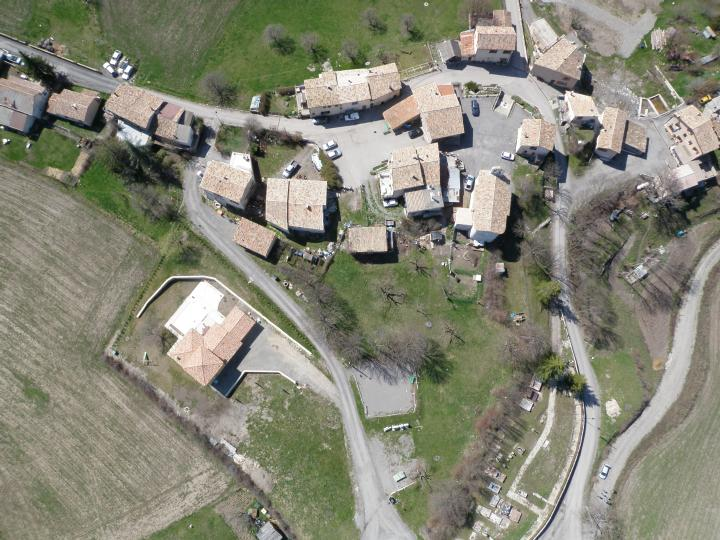
\includegraphics[width=45mm]{FIGS/TestOri/DraixIl.JPG}
\includegraphics[width=45mm]{FIGS/TestOri/DraixPx1.jpg}
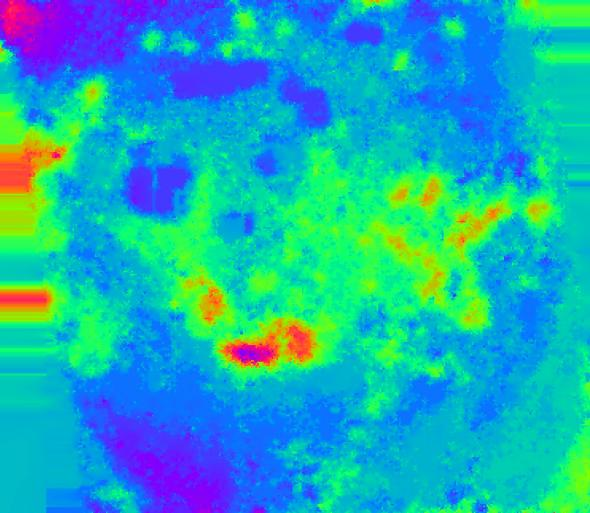
\includegraphics[width=45mm]{FIGS/TestOri/DraixPx2.jpg}
\end{center}
\caption{Image, depth map and transverse parallax with Draix data set
(images P4090163.JPG and P4090134.JPG)
}
\label{FIG:Draix:PxTr}
\end{figure}



\begin{figure}
\begin{center}
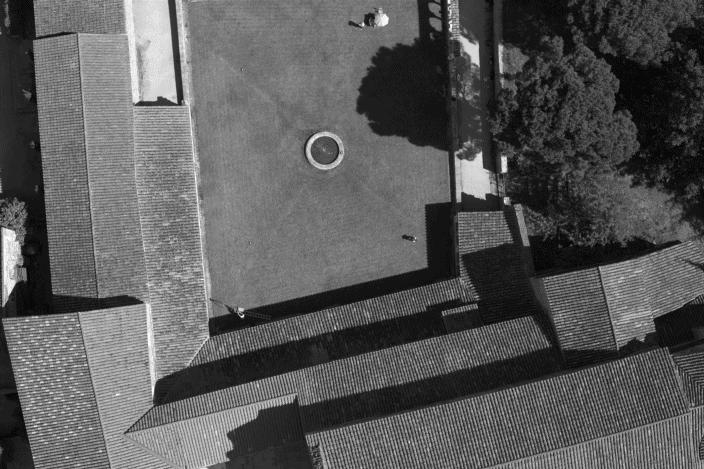
\includegraphics[width=45mm]{FIGS/TestOri/CuxIm.jpg}
\includegraphics[width=45mm]{FIGS/TestOri/CuxPx1.jpg}
\includegraphics[width=45mm]{FIGS/TestOri/CuxPx2.jpg}
\end{center}
\caption{Image, deptht map and transverse paralaxe with MiniCuxa data set
(images Abbey-IMG\_0208.jpg and Abbey-IMG\_0209.jpg), the correlation between two paralax
is lightly visible
}
\label{FIG:Cuxa:PxTr}
\end{figure}

\begin{figure}
\begin{center}
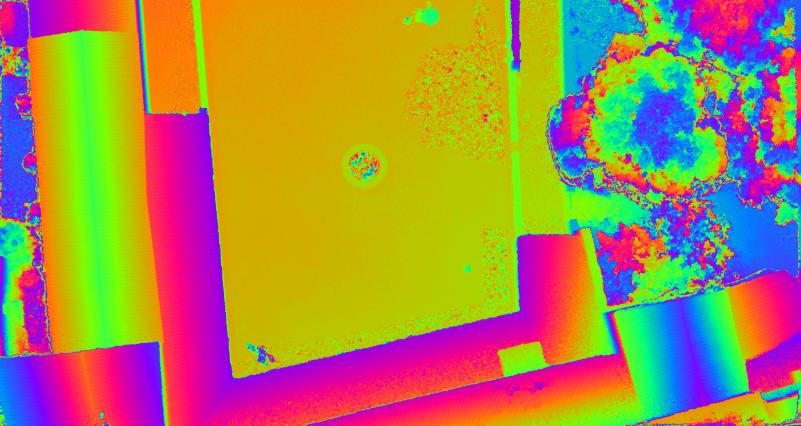
\includegraphics[width=60mm]{FIGS/TestOri/FullCuxPx1.jpg}
\includegraphics[width=60mm]{FIGS/TestOri/FullCuxPx2.jpg}
\end{center}
\caption{depth map and transverse parallax with full resolution Cuxa images,
correlation between both is clearly visible, amplitude is $\pm 1$ pixel.
}
\label{FIG:CuxaFull:PxTr}
\end{figure}


\begin{figure}
\begin{center}
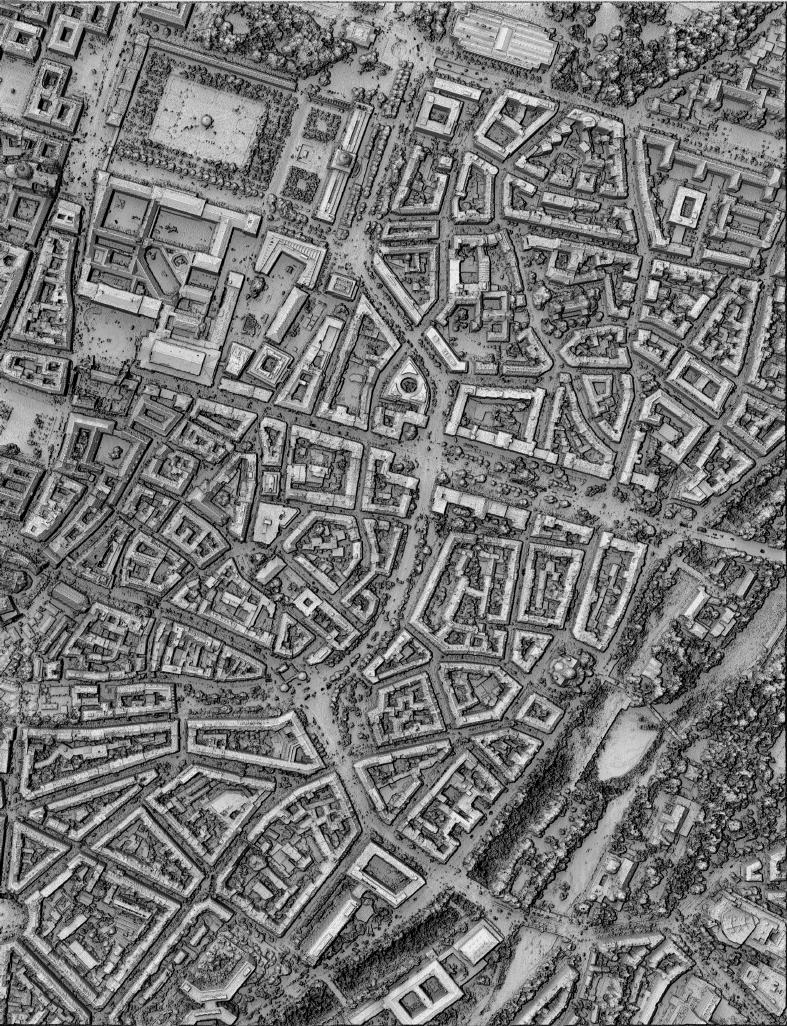
\includegraphics[width=60mm]{FIGS/TestOri/Mun1.jpg}
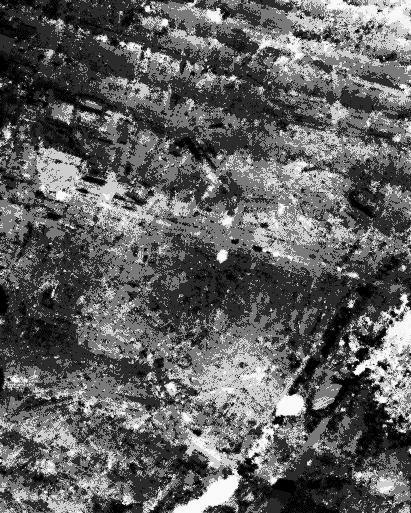
\includegraphics[width=60mm]{FIGS/TestOri/Mun2.jpg}
\end{center}
\caption{depth map and transverse parallax with $10$ cm image of Munich, acquired with a DMC,
except in "noisy part" like the river, amplitude of transverse parallax is $\pm\, 0.1$ pixel
}
\label{FIG:Mubich:PxTr}
\end{figure}




In image geometry {\tt MicMac} has "special" modes where the matching can be done
taking into account a possible inaccuracy of the orientation. Although, it can be used
to match badly oriented images, this is generally not a good idea (it's a better idea to
understand what was wrong in orientation or acquisition and to correct it !!). However,
when the user has doubts on orientation parameters, these tool can  be convenient to check
these orientations. In these mode :

\begin{itemize}
   \item the matching is done in image geometry : there is a master image, and the $X,Y$
         are the pixel of this master image;
   \item there is \emph{only} one secondary image;
   \item for each pixel of the master image, two value are computed, one represents the depths
         and the other represents the "transverse parallax" : it is the displacement in the direction
         orthogonal to the epipolar;
\end{itemize}

These mode can be fairly complex to use directly in {\tt XML} mode, so it's generally sufficient
to use the simplied tool {\tt MMTestOrient}. The  first arguments should be quite obvious from
inline help (argument after {\tt PB} are relative to satellite case, see~\ref{TestOri:PB}) :

\begin{verbatim}
mm3d MMTestOrient -help
*****************************
*  Help for Elise Arg main  *
*****************************
Unnamed args :
  * string :: {First Image}
  * string :: {Second Images}
  * string :: {Orientation}
Named args :
  * [Name=Dir] string :: {Directory, Def=./}
  * [Name=Zoom0] INT :: {Zoom init, pow of 2  in [128,8], Def depend of size}
  * [Name=ZoomF] INT :: {Zoom init,  pow of 2  in [4,1], Def=2}
  * [Name=PB] bool :: {Push broom sensor}
  * [Name=MOri] string :: {Mode Orientation (GRID or RTO) , Mandatory in PB}
  * [Name=ZMoy] REAL :: {Average Z,  Mandatory in PB}
  * [Name=ZInc] REAL :: {Incertitude on Z,  Mandatory in PB}
  * [Name=ShowCom] bool :: {Show MicMac command (tuning purpose)}
\end{verbatim}

The result of transverse parallaxes in stored in images {\tt Px2\dots}, the number of the last
and most accurate image depends of the other parameters, so you have to check what is
present on the directory {\tt GeoI-Px}.

How can these image be used ? Basically, the idea is that with a "perfect" orientation the
transverse parallax should be zero on all the image. In real life, this is more complicated, because this
parallax can be noisy ($2d$ general matching problem can be fairly ambiguous). So what is important is not
only the amplitude of the transverse parallax but also it spatial analysis : is there systematism in
this parallax ? Does it present low frequency movement ? Is this transverse parallax correlated to the
depth map ? \dots
It is not so easy to make an automatic quantitative analyze
of the results and the firt purpose of this tool is to help human expertise in a qualitative analysis of
the result.  The {\tt MMTestOrient} is illustrated on three examples (in each case with {\tt ZoomF=1}) :

\begin{itemize}
   \item on figure~\ref{FIG:Draix:PxTr} , with image from the Draix data set; in this case
          the transverse parallax is a bit noisy but does not show  obvious systematism;

   \item on figure~\ref{FIG:Cuxa:PxTr} , the amplitude of transverse parallax do not seem
         very high, but here it is computed on reduced images, and conversely one can guess
         some systematism and a correlation between the depth and the transverse parallax;

   \item on figure~\ref{FIG:CuxaFull:PxTr} ,  the full resolution image of Cuxa  have been
         used (they are not in the data-set); in this case, the tool show clearly a high systematism in
         the transverse parallax  , if we except the noisy part like the tree ~\footnote{for tree the
         transverse parallax can be created by wind} the amplitude in almost $\pm\,1$pixel
         between highest and lowest value; furthermore the high correlation between two parallax
         maybe originated by a calibration problem , probably due to focal length;

   \item figure~\ref{FIG:Mubich:PxTr} present an almost perfect orientation; with these $14144,15552$
         coming from a $DMC$ camera the amplitude of transverse parallax is $\pm\, 0.1$ pixel on most
         of the image; the only part of the image where the amplitude is significantly higher is
         the river, but as can be seen on the depth image, the matching is very noisy here and the
         result has meaning in such part;

\end{itemize}

\subsection{For Push-Broom Orientation}
\label{TestOri:PB}

This tool can be used also with satellite image :
\begin{itemize}
  \item in this case the third argument is interpreted as the postfix of the orientation file;
  \item the {\tt PB} argument must be set to true, indicating a push-broom sensor;
  \item the {\tt MOri} must indicate the way the orientation file is stored ({\tt GRID} for grid format,
       {\tt RTO} for  {\tt XML} encoded {\tt RPC} file;
  \item the {\tt ZMoy} must indicate the average value of $Z$;
  \item the {\tt ZInc} must indicate the incertitude on  $Z$;
\end{itemize}

Here is an example (in this case, the orientation file of {\tt ./crop1.tif} is {\tt ./crop1.GRIBin}) :

\begin{verbatim}
mm3d MMTestOrient  crop1.tif crop2.tif GRIBin PB=true MOri=GRID ZMoy=0 ZInc=1000
\end{verbatim}
%-------------------------------------------------------------------
%-------------------------------------------------------------------
%-------------------------------------------------------------------


\section{The Mars data-set}

\label{Mars}



\begin{figure}
\begin{center}
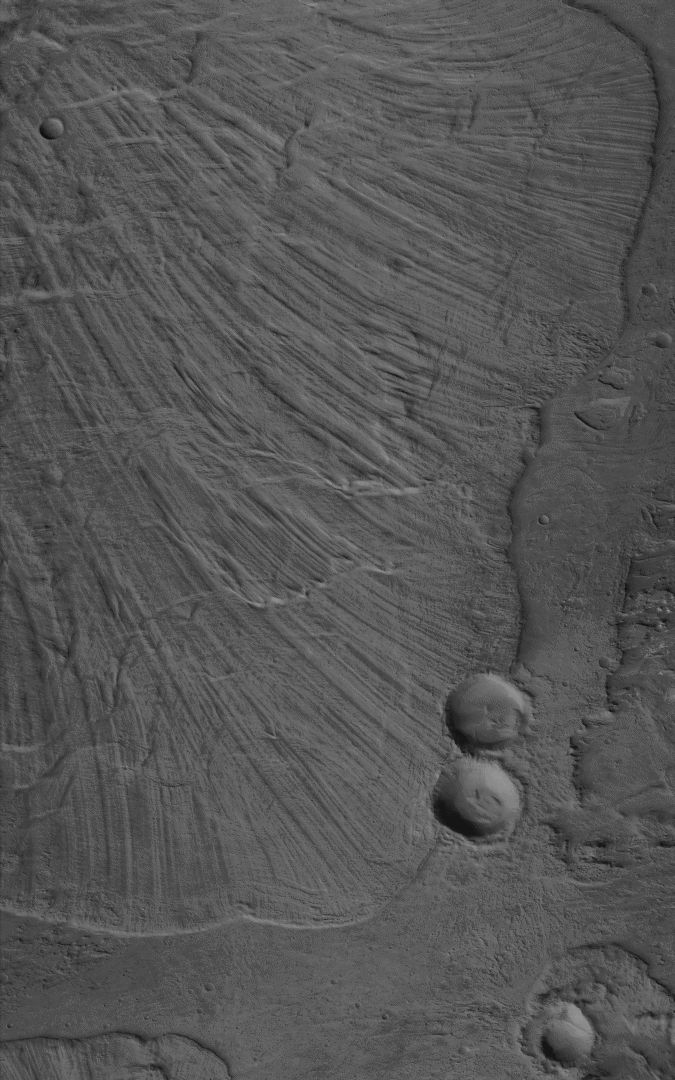
\includegraphics[width=35mm]{FIGS/Mars/SmaIm1.jpg}
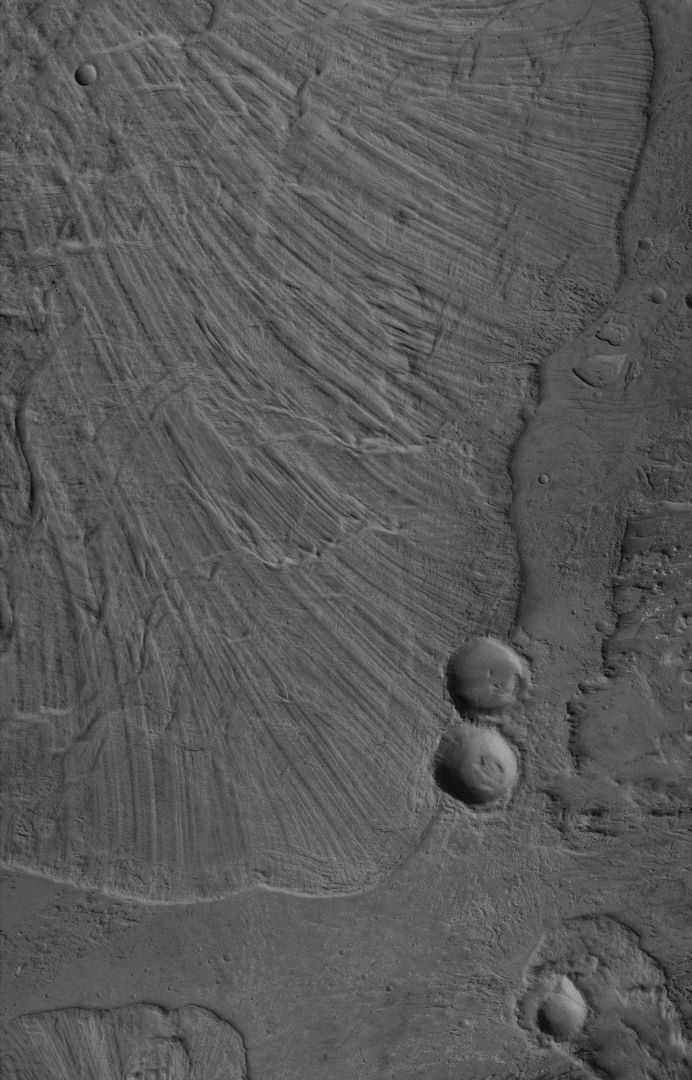
\includegraphics[width=35mm]{FIGS/Mars/SmIm2.jpg}
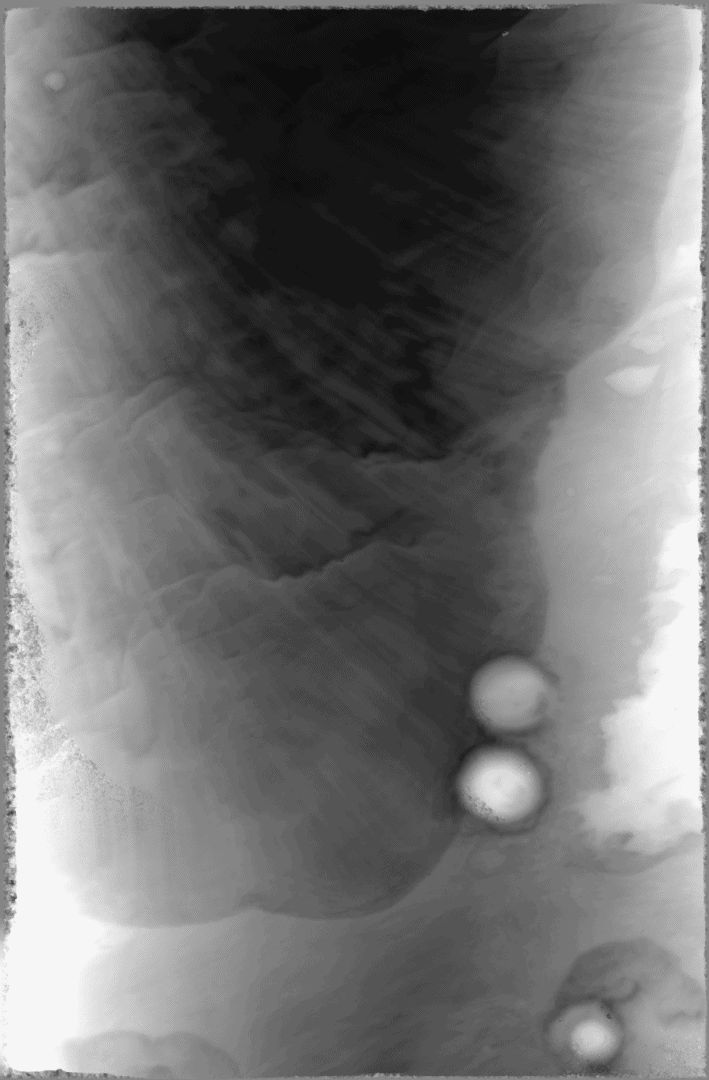
\includegraphics[width=35mm]{FIGS/Mars/Px1.jpg}
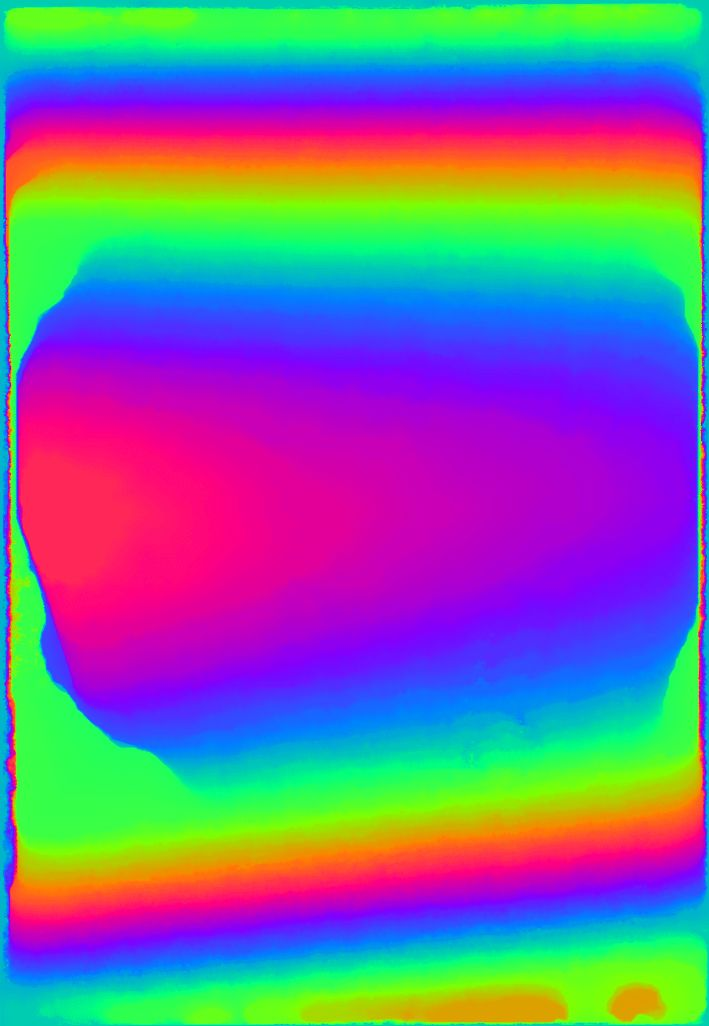
\includegraphics[width=35mm]{FIGS/Mars/Px2.jpg}

\end{center}
\caption{Mars data-set : the two  images, the $X$ parallax, in gray-level, and the $Y$-parallax in
hue color}
\label{FIG:OK:Mars}
\end{figure}



\subsection{Description of the data set}

The data can be found in the directory {\tt Mars/} of directory {\tt ExempleDoc/}.
It consists of two stereo images acquired by sensor CTX during MRO mission on the planet Mars. In this case
we do not have the physical model of the sensor, but we know that:

\begin{itemize}
   \item the satellite is a  pushbroom-satellite;
   \item it flights in the $x$ direction.
\end{itemize}

\subsection{Comment on the parameters}

\subsubsection{Geometry}

The tags controlling geometry are:

\begin{itemize}

   \item   {\tt <GeomImages> eGeomImage\_Hom\_Px </GeomImages>} indicates the geometry of the acquisition,
          here it means that there is a principal homography $H$, let $P_1=x_1,y_1$ and  $P_2=x_2,y_2$ be two
          homologous points, MicMac will compute $U(P_1)$ and $V(P_1)$ such that

\begin{equation}
    P_2 = H(P_1) + (U(P_1),V(P_1))
\end{equation}

   \item  the homography $H$ is computed by MicMac from a set of homologous point;

   \item  {\tt  <FCND\_CalcHomFromI1I2> NKS-Assoc-CplIm2Hom@-Man@xml  </FCND\_CalcHomFromI1I2>}  indicates
          where {\tt MicMac} must look for the tie points (see directory {\tt Homol-Man/});


   \item  {\tt <GeomMNT> eGeomPxBiDim  </GeomMNT>} indicates the geometry of restitution,
          the value {\tt eGeomPxBiDim} indicates that what is computed is the pixel offset, in fact this value
          is mandatory when using {\tt eGeomImage\_Hom\_Px}


\end{itemize}

\subsubsection{Matching}

In this case, the two parallax directions have completely different meanings:

\begin{itemize}
   \item the parallax $1$ represents mainly the relief, it is expected to contain high frequencies;
   \item the parallax $2$ represents mainly the error of the geometric model, it is expected to have
         low amplitude and low frequencies;
\end{itemize}

This asymmetry in the \emph{a priori} knowledge of parallax is specified at different parts of the file :

\begin{itemize}
   \item {\tt <Px1IncCalc>}   and {\tt <Px2IncCalc>},  representing the global uncertainty on each parallax;
   \item {\tt <Px1Regul>}   and {\tt <Px2Regul>},  representing the \emph{a priori} knowledge of the regularity of each
         parallax;
   \item {\tt <Px1PenteMax>}   and {\tt <Px2PenteMax>},  representing the \emph{a priori} knowledge of the
         \UNCLEAR{steep} of each parallax;
   \item {\tt <Px1Pas>}   and {\tt <Px2Pas>},  representing the discretization step (as Px2 is low frequency and
         low amplitude, we can compute it with higher precision);
   \item {\tt <Px1DilatAlti>}   and {\tt <Px2DilatAlti>}, to gain some time, we decide not to re-estimate Px2 at the last step;
\end{itemize}

\subsubsection{Results}

Figure~\ref{FIG:OK:Mars} presents the two images and the results of the computed parallax.
As expected:

\begin{itemize}
   \item The Px1 contains mainly high frequency information on the relief;
   \item The Px2 contains mainly low frequency information on  the geometry of the sensor.
\end{itemize}


%-------------------------------------------------------------------
%-------------------------------------------------------------------
\section{The Gulya Earthquake Data-Set}

\label{Gulya}

\subsection{Introduction}

Since September $2011$ CNES\footnote{Centre National d'Etudes Spatiales, the French spatial agency}
has been funding a development for using MicMac for  earthquake quantification. This development
was made as a collaboration between CNES, CEA, IPGP and IGN/ENSG. The main developer of this part
is Ana-Maria Rosu.

Although there exist other tools for doing this, the objective was:

\begin{itemize}
   \item have a totally free tool, that scientists can use in open source mode;
   \item have a more parametrizable tool;
\end{itemize}

Although the study is not finished, the tool  is now operational. The program has been
tested on $3$ real data set and several synthetic data set, and compared to several existing solutions
working in frequency domain. From a purely subjective evaluation, these tests show that the
results with MicMac are generally equivalent in quality to frequency approach and, on one of the
real data-set, the results of MicMac where "better"\footnote{i.e. subjectively easier to interpret
for scientist} . One of the drawback of the dense approach of
MicMac is the computation time : $15$ minutes, with a $8$ core computer, with the $1600*3600$
images of the Gulya data-set.


%-------------------------------------------------------------------

\subsection{Description of the data set}

The data can be found in the directory {\tt {SeismGuyla/}}
 of directory {\tt ExempleDoc/}. % micmac_data/ExempleDoc/
It consists of  two \emph{Spot 5} ortho photos of the same scene taken in $2002$ and
$2008$. Between these two dates, an earthquake occurred and image matching can be used to
localize the rupture and quantify the movement.

We want to use MicMac to measure very small displacements (around $\frac{1}{10}$ pixel) in
a context where the images are quite different. Figure~\ref{FIG:OK:Guylia} presents the two
ortho images.

\begin{figure}
\begin{center}
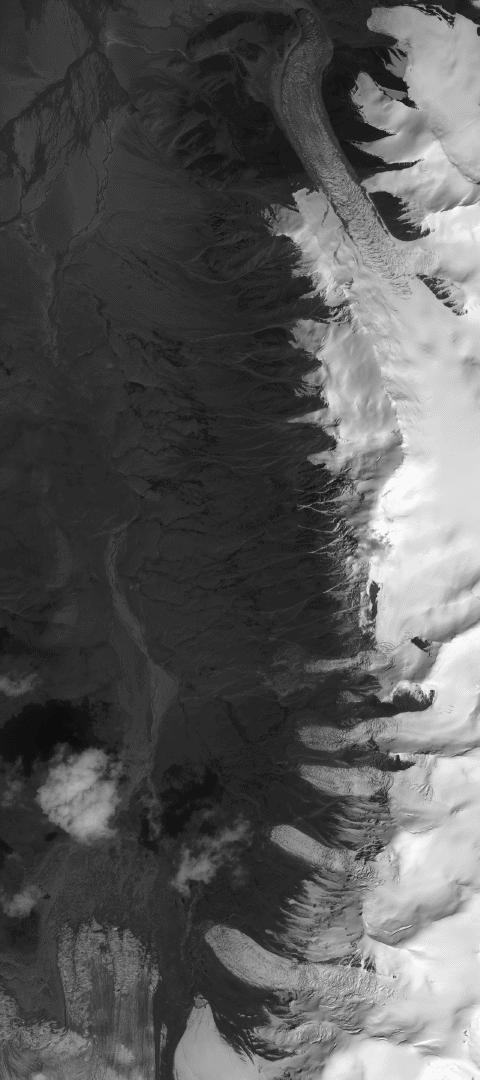
\includegraphics[width=35mm]{FIGS/SeismGuylia/250802_ortho.jpg}
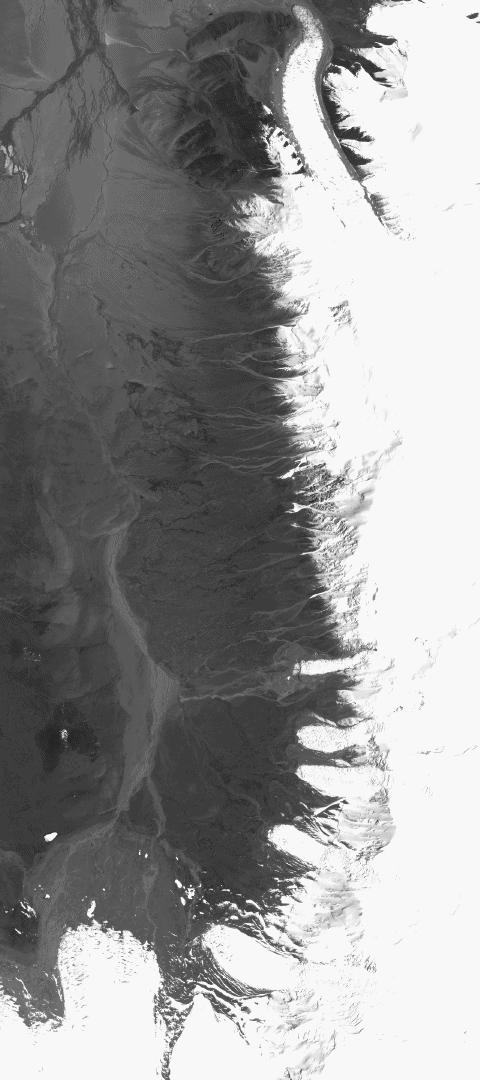
\includegraphics[width=35mm]{FIGS/SeismGuylia/260608_ortho.jpg}
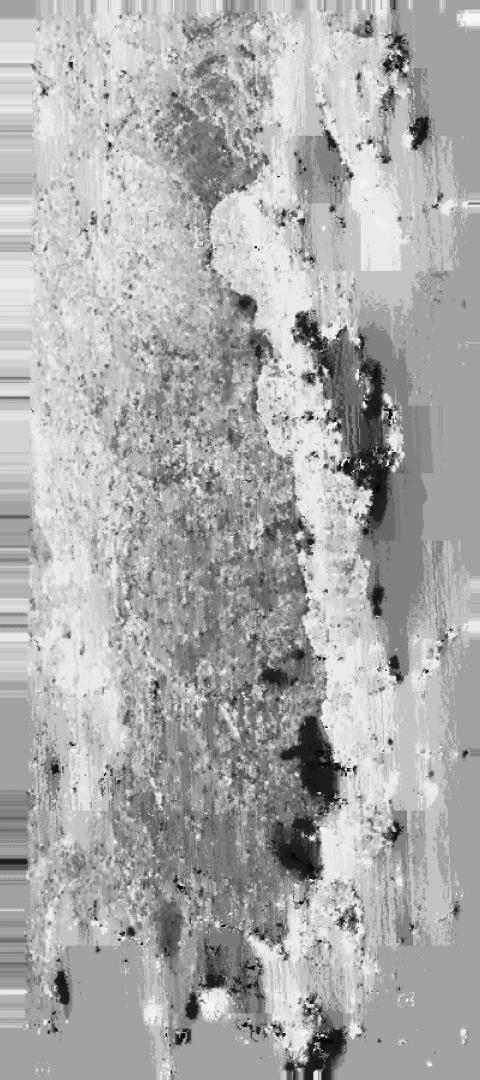
\includegraphics[width=35mm]{FIGS/SeismGuylia/Px1.jpg}
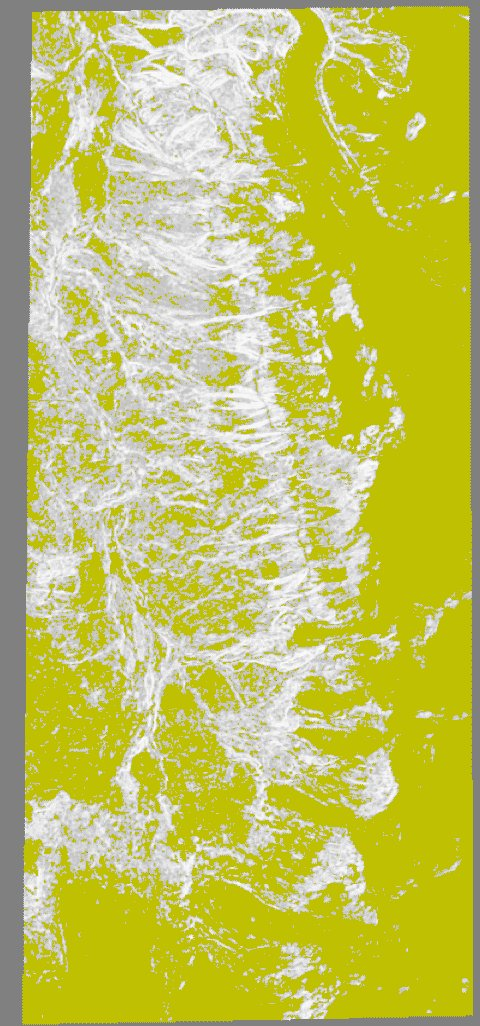
\includegraphics[width=35mm]{FIGS/SeismGuylia/Correl.jpg} %pourquoi la hauteur de l'image de correl est plus petite que le reste?

\end{center}
\caption{Guliya data set : the two ortho images, the $X$-parallax computed, and the correlation
coefficient computed}
\label{FIG:OK:Guylia}
\end{figure}


%-------------------------------------------------------------------
\subsection{Simplified interface}

A simplified interface has been written. At the time being, it gives acces to few parameters, but
it will evolve.

\begin{verbatim}
$ mm3d MM2DPosSism
*****************************
*  Help for Elise Arg main  *
*****************************
Unnamed args :
  * string :: {Image 1}
  * string :: {Image 2}
Named args :
  * [Name=Masq] string :: {Masq of focus zone (def=none)}
  * [Name=Teta] REAL :: {Direction of seism if any (in radian)}
  * [Name=Exe] bool :: {Execute command , def=true (tuning purpose)}
\end{verbatim}

An example of use :

\begin{verbatim}
    mm3d MM2DPosSism 250802_ortho.tif 260608_ortho.tif Teta=1.5
\end{verbatim}


%-------------------------------------------------------------------
\subsection{Comment on the parameters}

This section describes the "classical" interface using the {\tt XML} parameters.

\subsubsection{Interpolation}

Aiming at measuring very small displacements, we use a sinus cardinal interpolation :

\begin{itemize}
   \item {\tt <ModeInterpolation> eInterpolSinCard </ModeInterpolation>}

   \item  {\tt <SzSinCard>  5.0 </SzSinCard>} specifies the size of the kernel;

   \item  {\tt  <SzAppodSinCard>  5.0 </SzAppodSinCard>} controls the shape of the appodization
          window (the general shape is a Tukey window, when SzAppodSinCard=SzSinCard, it turns to be
          a Hamming window);
\end{itemize}


\subsubsection{Image term}

By default in MicMac, the image term is $1-Cor$ where $Cor$ is the normalized cross correlation
coefficient. In such data-sets, where there is a very important change locally, this can not be
suitable because when there are changes of the nature (snow \dots)  the correlation has no
signification and it is better to consider that there is no information. %pourquoi?
Three parameters are used here to control the meaning of the correlation:


\begin{itemize}
   \item {\tt  <CorrelMin> }=$C^{min}$ ,
         so  that correlation bellow $<C^{min}$ has no influence;
   \item {\tt  <GammaCorrel> }=$\gamma$, with $\gamma$ higher, higher is the influence of the correlation
         close to $1$;
   \item {\tt  <DynamiqueCorrel>=eCoeffGamma } to activate the previous one \dots
\end{itemize}

The following equations indicate how these parameters define the conversion from correlation to cost:

\begin{equation}
    C_1=Max(Cor,C^{min}) ,
\end{equation}

\begin{equation}
   C_2 = \frac{C_1 -C^{min}}{1-C^{min}}
\end{equation}

\begin{equation}
   C_3 = {C_2} ^\gamma
\end{equation}

\begin{equation}
   Cost  = (1-C_3) * (1-C^{min});
\end{equation}

On figure~\ref{FIG:OK:Guylia}, the image on the left presents the correlation coefficients. The yellow value corresponds to the threshold value (here $<0.5$).


\subsubsection{Non isotropic regularization}

It can happen that we have an \emph{a priori} knowledge for favoring some direction of regularization.
This can be done using in conjunction the following parameters of {\tt EtapeProgDyn}:

\begin{itemize}
   \item  {\tt  <NbDir>}=$N$  fixes the number of direction that will be explored;
   \item  {\tt  <Teta0>}=$\theta_0$  fixes the angle of the favored direction;
   \item  the directions that will be explored are $\alpha_k=\theta_0 + k\frac{\pi}{N} , k\in[0,N-1]$
   \item if the parameters  {\tt <Px1MultRegul>}=$V_1$ or {\tt <Px2MultRegul> } are used, then the value
         of regularization in the direction  $\alpha_k$ is  multiplied by $V_1[k]$ ($V_1$ is a vector);
\end{itemize}

In this example, we regularise more the direction close to $\frac{\pi}{2}$, with a weight
$\frac{1}{1+\frac{10}{N}*K}$.



%-------------------------------------------------------------------
%-------------------------------------------------------------------
\section{The Concrete Data-Set and civil engineering}

\label{Concrete}

\subsection{Introduction}

The data set {\tt Concrete/} is an example of using MicMac for measuring very fine displacement in civil engineering. In this experiment, constraint were applied to a concrete beam, and a fix camera was used to measure the displacement during breaking phase. Figure~\ref{FIG:OK:Concrete} illustrate this data set :

\begin{itemize}
    \item  (up left) a full view of on of the two images used for this correlation;
    \item  (up right) a zoom on a detail of this image, as it can be seen, the concrete a been
           painted to create an "optimal" texture for matching
    \item  (bottom left) the x displacement (total amplitude is around $\frac{1}{4}$ of pixel);
    \item  (bottom right) the y displacement (total amplitude is around $\frac{1}{4}$ of pixel).
\end{itemize}

\begin{figure}
\begin{center}
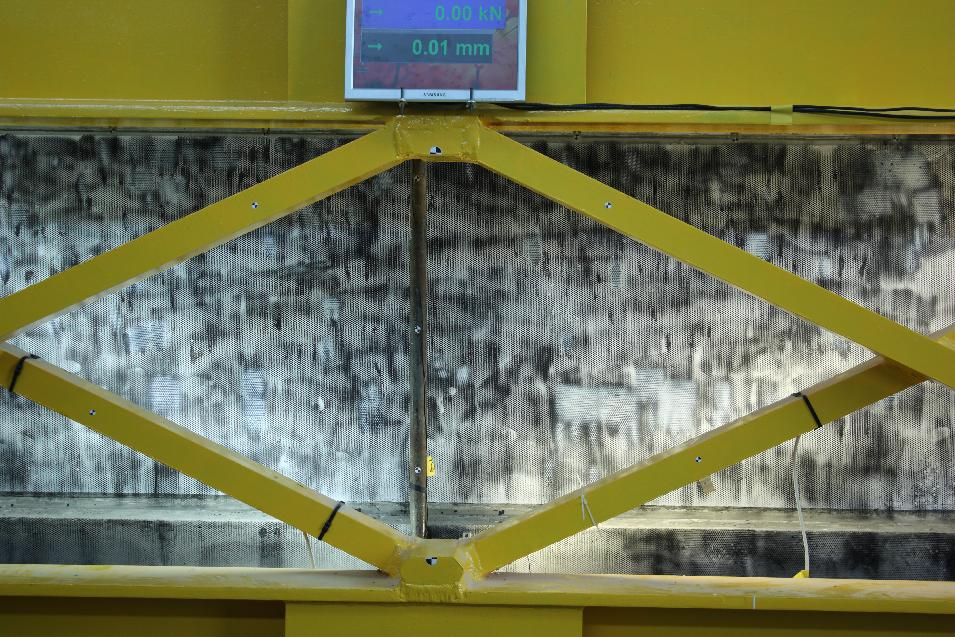
\includegraphics[width=74mm]{FIGS/Beton/IM1.jpg}
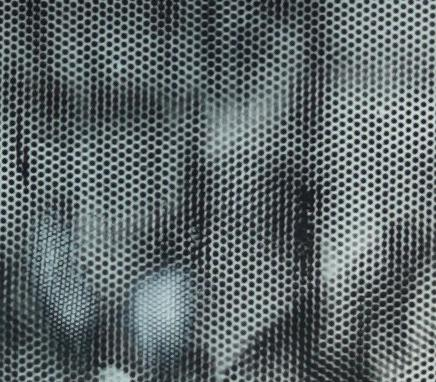
\includegraphics[width=56mm]{FIGS/Beton/IMCROP.jpg}

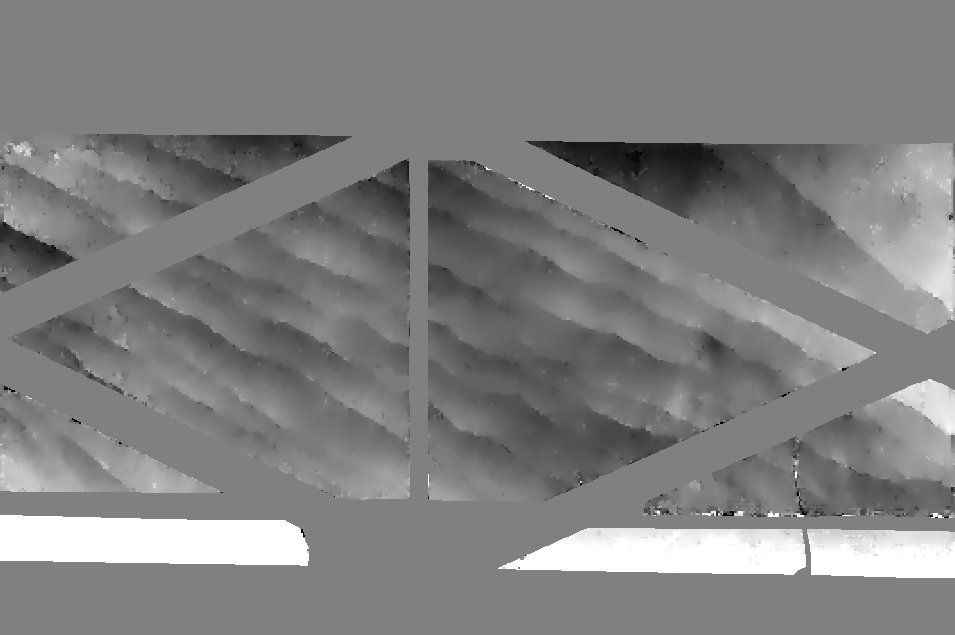
\includegraphics[width=65mm]{FIGS/Beton/Px1.jpg}
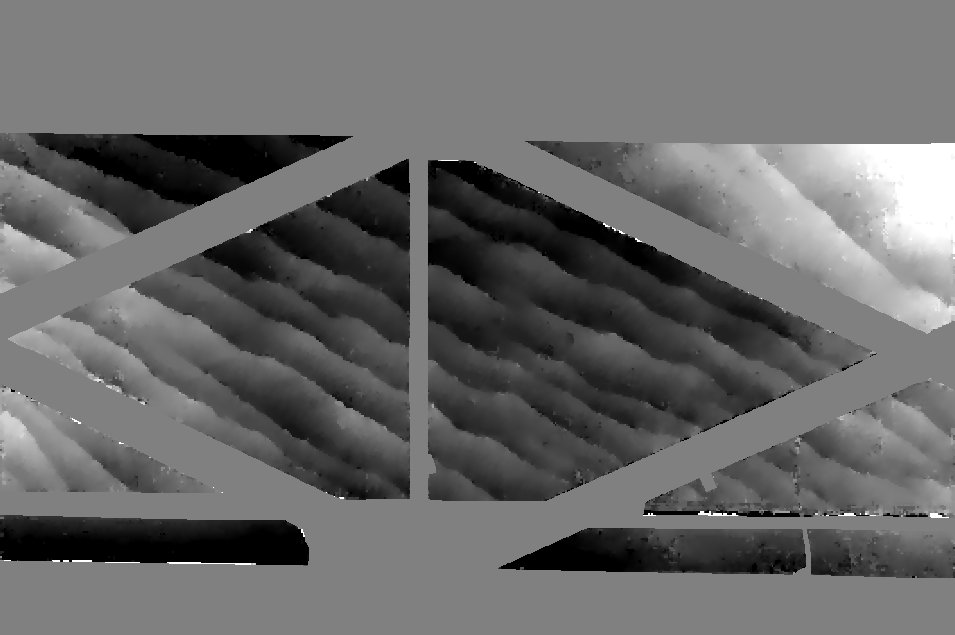
\includegraphics[width=65mm]{FIGS/Beton/Px2.jpg}

\end{center}
\caption{Concrete data'set, one of the image, a crop and the two displacement field}
\label{FIG:OK:Concrete}
\end{figure}

%-------------------------------------------------------------------

\subsection{Parametring}


The file {\tt Param-OneResol.xml} contain the MicMac's parametring used for this experience.
Although the parametring should be quite easy to understand after March's exemple, we can
do the following comments :

\begin{itemize}
    \item  the use of homographic model is well suited, it allow to model a possible translation
          of the camera; the $9$ point used for the homography have been seized on the concrete, this
          way the computed displacement is exactly the deformation;

    \item  we have not use the multi-scale approach because the quasi periodic texture uses was
           such that the reduced images where almost textureless at sub-resolution $8$ and very
           aliased at resolution $4$;
\end{itemize}


%-------------------------------------------------------------------
%-------------------------------------------------------------------
%~ \newpage

\section{FDSC - a post-processing tool for 2D correlation results}

\verb+FDSC+ (Fault Displacement Slip-Curve) is a post-processing tool. As \verb+MM2DPosSism+, it is also part of the collaboration between CNES, IPGP and IGN/ENSG, funded by CNES through the TOSCA program.

Mainly dedicated to the geoscience community, \verb+FDSC+ computes offsets by stacking profiles across the fault on the correlation results file and at the end, draws the slip-curve which gives an overview of the displacement field.

\verb+FDSC+ can be found in the MicMac deposit (folder \verb+fdsc/+). It is recommended to read the \verb+readme.txt+ before starting.

In order to launch \verb+FDSC+:
\begin{verbatim}
  ~/culture3d/fdsc$ ./fdsc.py
\end{verbatim}


The \verb+FDSC+'s \verb+Qt+ interface is divided into three main blocks corresponding to the three steps of FDSC:
\begin{enumerate}
  \item draw the fault trace
  \item stack profiles across the fault
  \item draw the slip-curve
\end{enumerate}

%-------------------------------------------------------------------

\subsection{Drawing the fault trace}

A polyline is drawn on a parallax image file (Px1 - epipolar parallax; Px2 - transverse parallax) to describe the fault trace. The parallax image used for this step has to have the same resolution as the parallax images used when stacking, otherwise the fault trace is useless.

A file containing the points of the polyline describing the fault is saved (e.g. \verb+trace.txt+) and later used to retrieve the fault when stacking profiles.
The first drawn point of the fault trace (Fig. \ref{FIG:fdsc_traceFaultK_withFrames}) is considered to be the fault origin. The drawing direction is the fault direction. %the orientation of the fault defines the fault orientation for measurements of parallel and normal to the fault displacements

\begin{figure}
  \begin{center}
    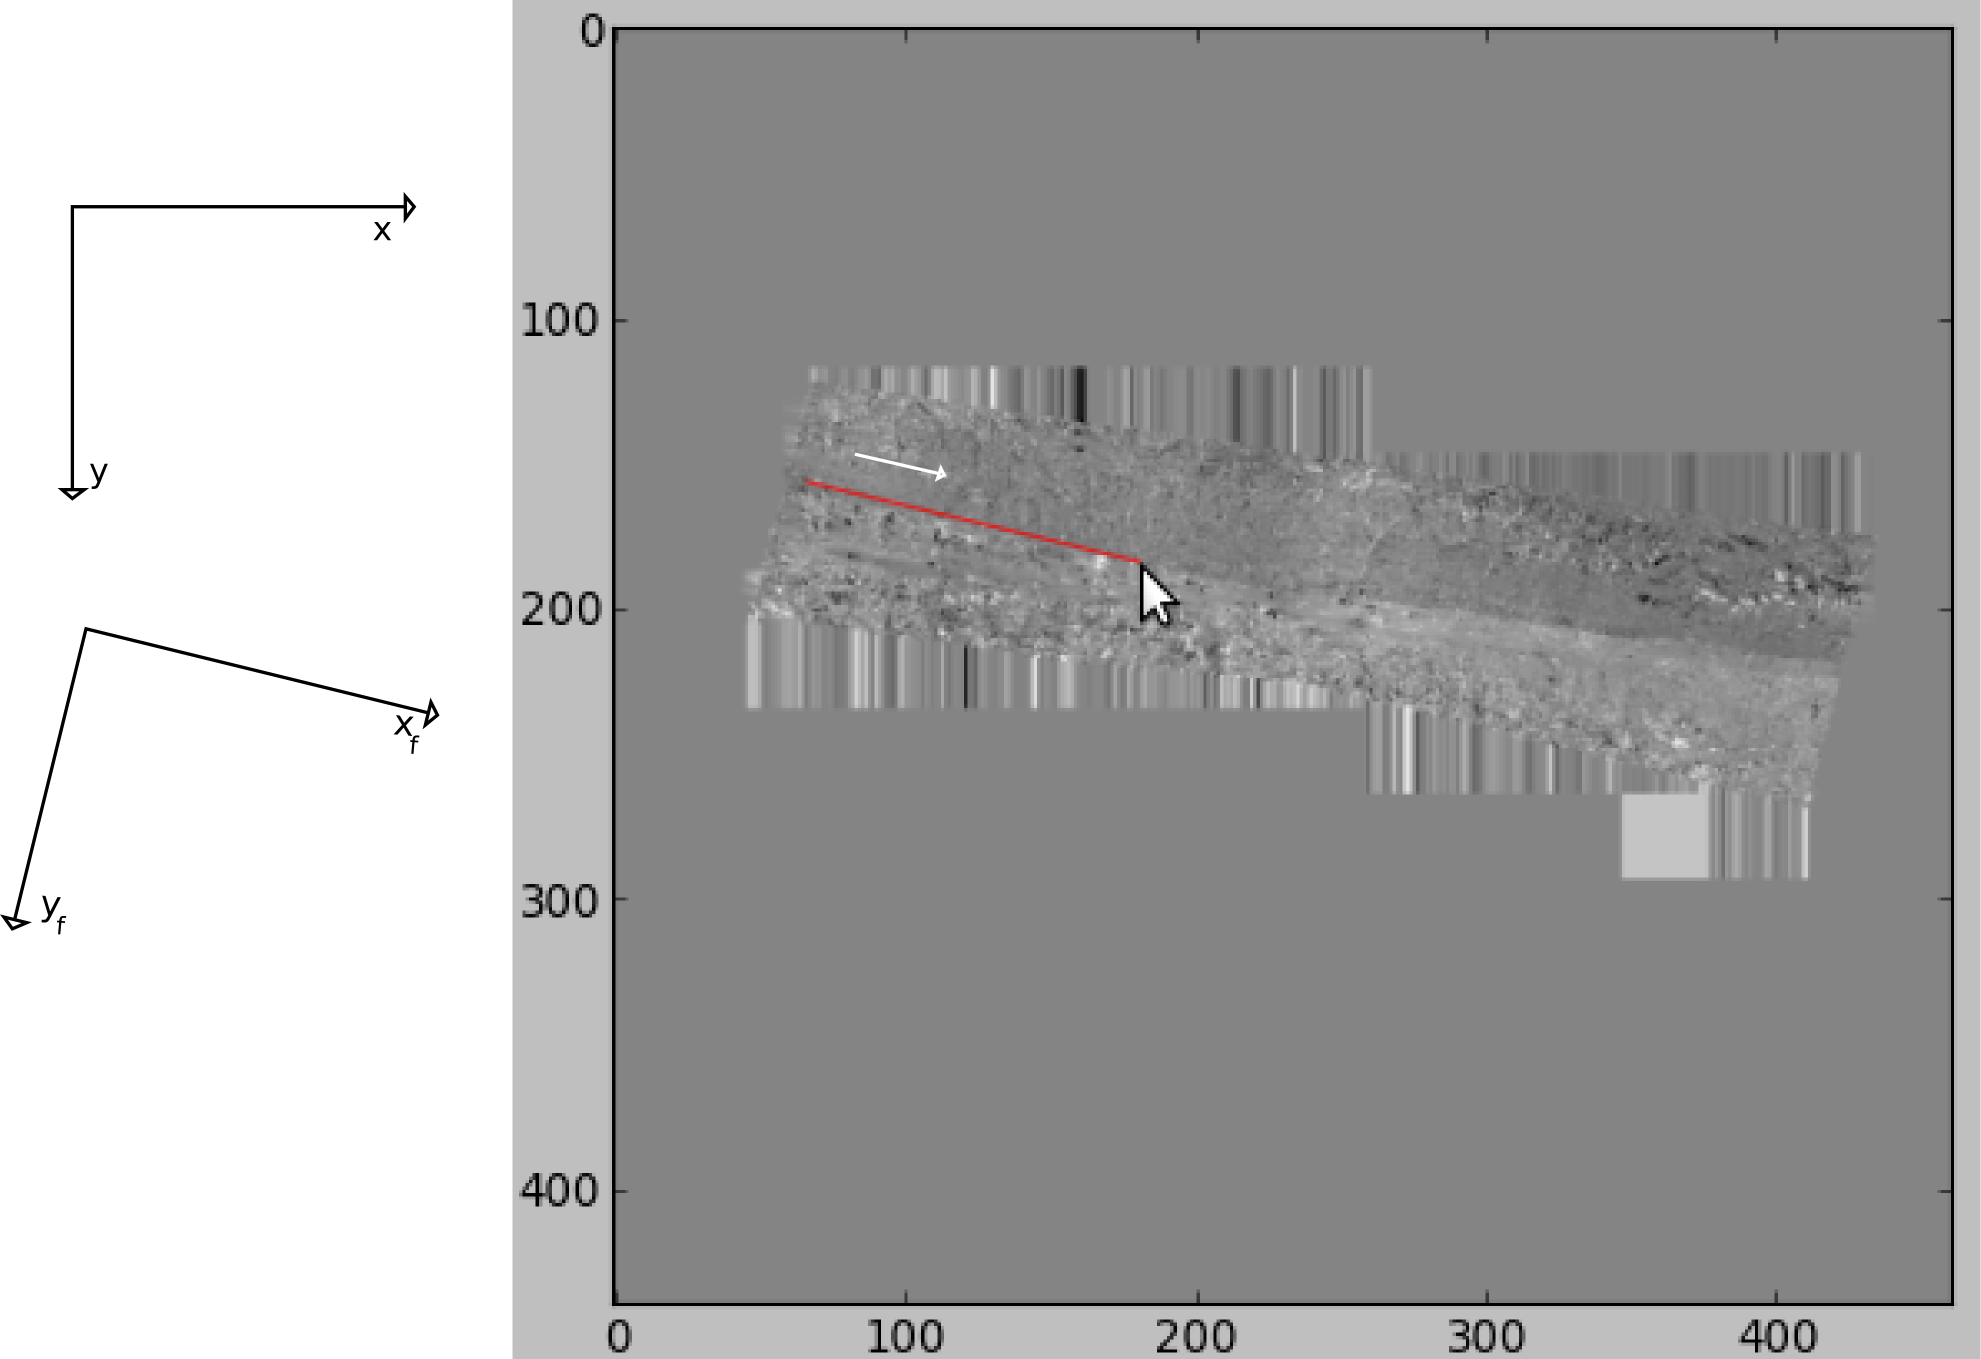
\includegraphics[width=0.6\textwidth]{FIGS/Fdsc/fdsc_traceFaultK_withFrames.png}
  \end{center}
  \caption{FDSC - drawing the fault trace; $uv$ - image reference frame ($\vec{u}$ - in epipolar direction, $\vec{v}$ - in transverse direction); $u_fv_f$ - fault reference frame ($\vec{u_f}$ - parallel to the fault line, $\vec{v_f}$ - perpendicular to the fault line)}
  \label{FIG:fdsc_traceFaultK_withFrames}
\end{figure}

%-------------------------------------------------------------------

\subsection{Stacking profiles}

Perpendicular profiles \UNCLEAR{(direction from left to right from the fault direction)} are stacked to obtain the fault offsets.
\UNCLEAR{A stack of profiles is composed of numerous single profiles. The result is a ``mean profile'' where the noise is diminished and the offset trend comes out very well, making it easier to measure (see Fig. \ref{FIG:demo_interetStack}).}

\begin{figure}%[h!]
  \begin{center}
  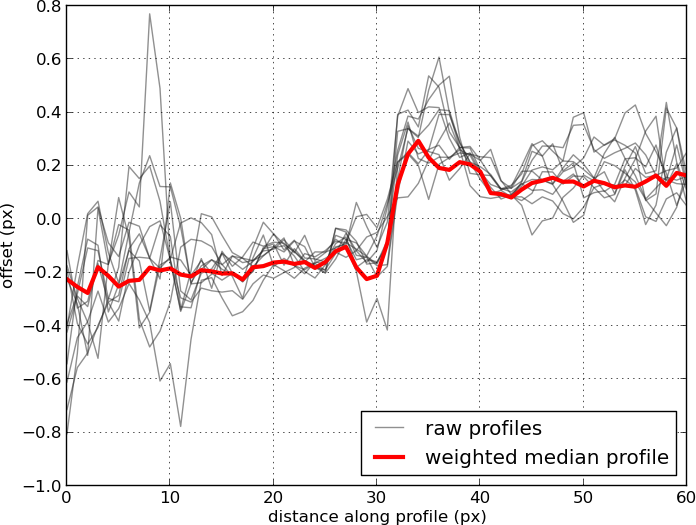
\includegraphics[width=0.5\textwidth]{FIGS/Fdsc/demo_interetStack.png}
  \caption{Single (raw) profiles perpendicular to the fault and a resulted stack}
  \label{FIG:demo_interetStack}
  \end{center}
\end{figure}

Parameters defining a stack:
\begin{itemize}
  \item computing method: mean or weighted mean, median or weighted median of profiles;
  \item when a weighted method is chosen, the values of the correlation coefficients' image are considered as weights (these values express well the confidence in the corresponding parallax values), therefore  the user must indicate the correlation coefficients' image,a s well as the value of the exponent of weights.
  \item width : number of profiles taken into account, 1 pixel apart (it must be a odd number)
  \item length : length of profiles, in pixels (it must be a odd number)
  \item profile projection or offsets output direction: ``Column'', ``Line'' (corresponding to $u$ projection - only Px1 image is used and $v$ projection respectively - only Px2 is used in stacks computation); ``Parallel'', ``Perpendicular'' (profiles are projected in the fault parallel, $u_f$, and fault normal direction, $v_f$, respectively; both Px1 and Px2 images are needed for stacks computation).
\end{itemize}

The offsets values are saved into a file (e.g \verb++offsets.txt++ to which a suffix is added by default depending on the chosen projection: $offsets\_dirCol.txt$,  $offsets\_dirLine.txt$, $offsets\_dirParal.txt$, $offsets\_dirPerp.txt$).

\subsection{Drawing the slip-curve}
The input file needed is the offsets output file and the slip curve will be drawn accordingly to these values.




